\documentclass[a4paper,14pt]{extreport}
\usepackage[left=1.5cm,right=1.5cm,
    top=1.5cm,bottom=2cm,bindingoffset=0cm]{geometry}
\usepackage{scrextend}
\usepackage[T1,T2A]{fontenc}
\usepackage[utf8]{inputenc}
\usepackage[english,russian,ukrainian]{babel}
\usepackage{tabularx}
\usepackage{amssymb}
\usepackage{color}
\usepackage{amsmath}
\usepackage{mathrsfs}
\usepackage{listings}
\usepackage{graphicx}
\graphicspath{ {./images/} }
\usepackage{lipsum}
\usepackage{xcolor}
\usepackage{hyperref}
\usepackage{tcolorbox}
\usepackage{tikz}
\usepackage[framemethod=TikZ]{mdframed}
\usepackage{wrapfig,boxedminipage,lipsum}
\mdfdefinestyle{MyFrame}{%
linecolor=blue,outerlinewidth=2pt,roundcorner=20pt,innertopmargin=\baselineskip,innerbottommargin=\baselineskip,innerrightmargin=20pt,innerleftmargin=20pt,backgroundcolor=gray!50!white}
 \usepackage{csvsimple}
 \usepackage{supertabular}
\usepackage{pdflscape}
\usepackage{fancyvrb}
%\usepackage{comment}
\usepackage{array,tabularx}
\usepackage{colortbl}

\usepackage{varwidth}
\tcbuselibrary{skins}
\usepackage{fancybox}


\usepackage{tikz}
\usepackage[framemethod=TikZ]{mdframed}
\usepackage{xcolor}
\usetikzlibrary{calc}
\makeatletter
\newlength{\mylength}
\xdef\CircleFactor{1.1}
\setlength\mylength{\dimexpr\f@size pt}
\newsavebox{\mybox}
\newcommand*\circled[2][draw=blue]{\savebox\mybox{\vbox{\vphantom{WL1/}#1}}\setlength\mylength{\dimexpr\CircleFactor\dimexpr\ht\mybox+\dp\mybox\relax\relax}\tikzset{mystyle/.style={circle,#1,minimum height={\mylength}}}
\tikz[baseline=(char.base)]
\node[mystyle] (char) {#2};}
\makeatother

\definecolor{ggreen}{rgb}{0.4,1,0}
\definecolor{rred}{rgb}{1,0.1,0.1}
\definecolor{amber}{rgb}{1.0, 0.75, 0.0}
\definecolor{babyblue}{rgb}{0.54, 0.81, 0.94}
\definecolor{asparagus}{rgb}{0.53, 0.66, 0.42}
\definecolor{chartreuse}{rgb}{0.5, 1.0, 0.0}
\definecolor{darkorchid}{rgb}{0.6, 0.2, 0.8}

\usepackage{float}
\usepackage{wrapfig}
\usepackage{framed}
%for nice Code{
\lstdefinestyle{customc}{
  belowcaptionskip=1\baselineskip,
  breaklines=true,
  frame=L,
  xleftmargin=\parindent,
  language=C,
  showstringspaces=false,
  basicstyle=\small\ttfamily,
  keywordstyle=\bfseries\color{green!40!black},
  commentstyle=\itshape\color{purple!40!black},
  identifierstyle=\color{blue},
  stringstyle=\color{orange},
}
\lstset{escapechar=@,style=customc}
%}


\begin{document}
\pagecolor{white}

%----------------------------------------1
\newtcbox{\xmybox}[1][red]{on line, arc=7pt,colback=#1!10!white,colframe=#1!50!black, before upper={\rule[3pt] {0pt}{10pt}},boxrule=1pt,boxsep=0pt,left=6pt,right=6pt,top=2pt,bottom=2pt}

\begin{center}Bohdan Lyshchenko DP-82 Variant №4
\vspace{1cm}

\end{center}


\begin{center}Як математично і графічно описуються діелектричні втрати від провідності?\end{center}


During the directed movement of electric charges in an external electric field (drift or diffusion), the charge carriers receive energy from the
electric field in the free path path. Acquired energy is lost due to "collisions" - interactions with molecules and atoms of matter that are in a state of thermal motion. By giving off energy during collisions, the charge carrier increases the intensity of the chaotic motion of the particles of matter, and thus increases the temperature of the dielectric. As a result, the electrical conductivity increases the value of the loss factor
$\varepsilon$", the tangent of the loss angle $tg \delta$ and the power of energy dissipation p per unit volume of the dielectric.
All these parameters depend only on the density of the active current flowing through the dielectric. From the corresponding formulas given below, it follows that the electrical conductivity affects the value of tg and the loss factor $\varepsilon$ "mostly at low frequencies: these two parameters decrease depending on the frequency as 1/$\omega$. The specific power loss in this case does not depend on the frequency, DC voltage (p = aE$^2$). Therefore, a decrease in $\varepsilon$ and $tg \delta$ with increasing frequency does not mean a decrease in heat dissipation in the dielectric, because the loss parameter p is directly proportional to the frequency $\omega$.


The frequency characteristics of the considered paramert are shown in fig. 1, a.
 The dielectric constant due to (if there are no other absorption mechanisms other
 than electrical conductivity) only fast polarization processes, $\varepsilon = \varepsilon(\infty)$,
 and does not depend on the frequency. Both $tg \delta$ and $\varepsilon$ decrease with increasing
 frequency, but the value of the specific power of losses p is constant.
The temperature dependences of these parameters in the case of a predominance of electrical conductivity
are shown in fig. 1, b. All of them increase exponentially with increasing temperature, because according
to this law, the conductivity also changes. It is seen that the electrical conductivity makes a significant
 contribution to $tg \delta$ and $\varepsilon$ at high temperatures and low frequencies. At low temperatures
  and rather high frequencies the contribution of electrical conductivity to dielectric losses can be neglected.




\begin{figure}[h]
\center{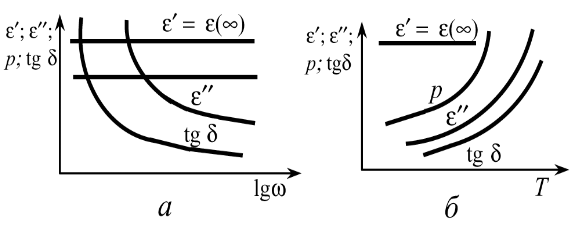
\includegraphics[width=0.6\linewidth]{1.png}}
\caption{Frequency (a) and temperature (b) dependences of the basic parameters of a dielectric in which losses of conductivity prevail.}
\label{ris1}
\end{figure}
\end{document}
